% Options for packages loaded elsewhere
\PassOptionsToPackage{unicode}{hyperref}
\PassOptionsToPackage{hyphens}{url}
%
\documentclass[
]{article}
\usepackage{amsmath,amssymb}
\usepackage{lmodern}
\usepackage{iftex}
\ifPDFTeX
  \usepackage[T1]{fontenc}
  \usepackage[utf8]{inputenc}
  \usepackage{textcomp} % provide euro and other symbols
\else % if luatex or xetex
  \usepackage{unicode-math}
  \defaultfontfeatures{Scale=MatchLowercase}
  \defaultfontfeatures[\rmfamily]{Ligatures=TeX,Scale=1}
\fi
% Use upquote if available, for straight quotes in verbatim environments
\IfFileExists{upquote.sty}{\usepackage{upquote}}{}
\IfFileExists{microtype.sty}{% use microtype if available
  \usepackage[]{microtype}
  \UseMicrotypeSet[protrusion]{basicmath} % disable protrusion for tt fonts
}{}
\makeatletter
\@ifundefined{KOMAClassName}{% if non-KOMA class
  \IfFileExists{parskip.sty}{%
    \usepackage{parskip}
  }{% else
    \setlength{\parindent}{0pt}
    \setlength{\parskip}{6pt plus 2pt minus 1pt}}
}{% if KOMA class
  \KOMAoptions{parskip=half}}
\makeatother
\usepackage{xcolor}
\IfFileExists{xurl.sty}{\usepackage{xurl}}{} % add URL line breaks if available
\IfFileExists{bookmark.sty}{\usepackage{bookmark}}{\usepackage{hyperref}}
\hypersetup{
  pdftitle={Confidence Level Project},
  pdfauthor={Shishir Katta, Nick Huo, Yida Chen},
  hidelinks,
  pdfcreator={LaTeX via pandoc}}
\urlstyle{same} % disable monospaced font for URLs
\usepackage[margin=1in]{geometry}
\usepackage{color}
\usepackage{fancyvrb}
\newcommand{\VerbBar}{|}
\newcommand{\VERB}{\Verb[commandchars=\\\{\}]}
\DefineVerbatimEnvironment{Highlighting}{Verbatim}{commandchars=\\\{\}}
% Add ',fontsize=\small' for more characters per line
\usepackage{framed}
\definecolor{shadecolor}{RGB}{248,248,248}
\newenvironment{Shaded}{\begin{snugshade}}{\end{snugshade}}
\newcommand{\AlertTok}[1]{\textcolor[rgb]{0.94,0.16,0.16}{#1}}
\newcommand{\AnnotationTok}[1]{\textcolor[rgb]{0.56,0.35,0.01}{\textbf{\textit{#1}}}}
\newcommand{\AttributeTok}[1]{\textcolor[rgb]{0.77,0.63,0.00}{#1}}
\newcommand{\BaseNTok}[1]{\textcolor[rgb]{0.00,0.00,0.81}{#1}}
\newcommand{\BuiltInTok}[1]{#1}
\newcommand{\CharTok}[1]{\textcolor[rgb]{0.31,0.60,0.02}{#1}}
\newcommand{\CommentTok}[1]{\textcolor[rgb]{0.56,0.35,0.01}{\textit{#1}}}
\newcommand{\CommentVarTok}[1]{\textcolor[rgb]{0.56,0.35,0.01}{\textbf{\textit{#1}}}}
\newcommand{\ConstantTok}[1]{\textcolor[rgb]{0.00,0.00,0.00}{#1}}
\newcommand{\ControlFlowTok}[1]{\textcolor[rgb]{0.13,0.29,0.53}{\textbf{#1}}}
\newcommand{\DataTypeTok}[1]{\textcolor[rgb]{0.13,0.29,0.53}{#1}}
\newcommand{\DecValTok}[1]{\textcolor[rgb]{0.00,0.00,0.81}{#1}}
\newcommand{\DocumentationTok}[1]{\textcolor[rgb]{0.56,0.35,0.01}{\textbf{\textit{#1}}}}
\newcommand{\ErrorTok}[1]{\textcolor[rgb]{0.64,0.00,0.00}{\textbf{#1}}}
\newcommand{\ExtensionTok}[1]{#1}
\newcommand{\FloatTok}[1]{\textcolor[rgb]{0.00,0.00,0.81}{#1}}
\newcommand{\FunctionTok}[1]{\textcolor[rgb]{0.00,0.00,0.00}{#1}}
\newcommand{\ImportTok}[1]{#1}
\newcommand{\InformationTok}[1]{\textcolor[rgb]{0.56,0.35,0.01}{\textbf{\textit{#1}}}}
\newcommand{\KeywordTok}[1]{\textcolor[rgb]{0.13,0.29,0.53}{\textbf{#1}}}
\newcommand{\NormalTok}[1]{#1}
\newcommand{\OperatorTok}[1]{\textcolor[rgb]{0.81,0.36,0.00}{\textbf{#1}}}
\newcommand{\OtherTok}[1]{\textcolor[rgb]{0.56,0.35,0.01}{#1}}
\newcommand{\PreprocessorTok}[1]{\textcolor[rgb]{0.56,0.35,0.01}{\textit{#1}}}
\newcommand{\RegionMarkerTok}[1]{#1}
\newcommand{\SpecialCharTok}[1]{\textcolor[rgb]{0.00,0.00,0.00}{#1}}
\newcommand{\SpecialStringTok}[1]{\textcolor[rgb]{0.31,0.60,0.02}{#1}}
\newcommand{\StringTok}[1]{\textcolor[rgb]{0.31,0.60,0.02}{#1}}
\newcommand{\VariableTok}[1]{\textcolor[rgb]{0.00,0.00,0.00}{#1}}
\newcommand{\VerbatimStringTok}[1]{\textcolor[rgb]{0.31,0.60,0.02}{#1}}
\newcommand{\WarningTok}[1]{\textcolor[rgb]{0.56,0.35,0.01}{\textbf{\textit{#1}}}}
\usepackage{graphicx}
\makeatletter
\def\maxwidth{\ifdim\Gin@nat@width>\linewidth\linewidth\else\Gin@nat@width\fi}
\def\maxheight{\ifdim\Gin@nat@height>\textheight\textheight\else\Gin@nat@height\fi}
\makeatother
% Scale images if necessary, so that they will not overflow the page
% margins by default, and it is still possible to overwrite the defaults
% using explicit options in \includegraphics[width, height, ...]{}
\setkeys{Gin}{width=\maxwidth,height=\maxheight,keepaspectratio}
% Set default figure placement to htbp
\makeatletter
\def\fps@figure{htbp}
\makeatother
\setlength{\emergencystretch}{3em} % prevent overfull lines
\providecommand{\tightlist}{%
  \setlength{\itemsep}{0pt}\setlength{\parskip}{0pt}}
\setcounter{secnumdepth}{-\maxdimen} % remove section numbering
\ifLuaTeX
  \usepackage{selnolig}  % disable illegal ligatures
\fi

\title{Confidence Level Project}
\author{Shishir Katta, Nick Huo, Yida Chen}
\date{2022-04-07}

\begin{document}
\maketitle

\hypertarget{install-all-libraries}{%
\subsection{Install all libraries}\label{install-all-libraries}}

\begin{Shaded}
\begin{Highlighting}[]
\CommentTok{\#install.packages("ggplot2")}
\end{Highlighting}
\end{Shaded}

\begin{Shaded}
\begin{Highlighting}[]
\FunctionTok{library}\NormalTok{(ggplot2)}
\end{Highlighting}
\end{Shaded}

\hypertarget{welcome-to-our-introduction-of-confidence-level}{%
\subsection{\texorpdfstring{1 Welcome to our introduction of Confidence
Level!\\
}{1 Welcome to our introduction of Confidence Level! }}\label{welcome-to-our-introduction-of-confidence-level}}

In this project, we will cover the concepts of repeated sampling,
confidence levels and intervals. We will introduce the concepts through
both the texts and visualizations.

Before reaching these goals, we need to review several key concepts that
are fundamental for the study of confidence levels.

\hypertarget{sampling-distribution}{%
\subsubsection{1.1 Sampling Distribution}\label{sampling-distribution}}

The sampling distribution is the probability distribution of a statistic
(e.g.~mean) calculated from different experiments. Each experiment will
randomly draw a number of samples from the population. All data of the
population have the same probability of being chosen by the experiment.

\hypertarget{central-limit-theorem}{%
\subsubsection{1.2 Central Limit Theorem}\label{central-limit-theorem}}

Why is sampling distribution important? According to the Central Limit
Theorem (CLT), if we have random samples, \(X_1, \ X_2, \dots, X_n\),
from a population with mean \(\mu\) and standard deviation \(\sigma\),
and if the sample size \(n\) is sufficiently large, then the
distribution of the sample mean \(\bar{x}\) is approximately normal with
mean \(\mu\) and standard deviation \(\frac{\sigma}{\sqrt{n}}\).

\[\bar{X} \approx \mathcal{N}\left(\mu, \frac{\sigma}{\sqrt{n}}\right)\]

This is true regardless the shape of the population distribution. In
other words, the shape of sampling distribution of \(\bar{X}\) will be
approximately normal (for large sample size \(n\)) even if the
population distribution is not.

\hypertarget{what-are-the-confidence-level-and-confidence-interval}{%
\subsection{2. What are the confidence level and confidence
interval?}\label{what-are-the-confidence-level-and-confidence-interval}}

After this quick review of the sampling distribution and CLT, we now can
start our exploration of confidence level and interval.

What are the confidence level and interval? In simple words, the
confidence level represents the proportion of the time that its
associated interval calculated from samples will capture the true
parameters, namely, the success rate. For example with a 90\% confidence
interval for the mean, you would expect the intervals calculated from
the 90\% of experiments with \(n\) random samples will cover the true
population mean.

A confidence interval is useful when we want to find a possible range of
a population parameter but only a sample of the population is available.
We use the sampled observations, which may be a good approximation of
population distribution, to estimate a possible range for the true
parameter.

The population parameter (e.g.~mean or median) is a fixed value, but the
sample statistic is a random variable because we are uncertain about its
value before obtaining the samples. Thus, the intervals calculated with
sample statistics may or may not contain the true parameter. The
intervals' long-run success rate of capturing true parameters is
determined by their confidence level.

\hypertarget{understanding-intervals}{%
\subsection{3. Understanding intervals}\label{understanding-intervals}}

The confidence interval is a range of possible values for a population
parameter. It is calculated from a set of samples. For a confidence
interval of mean, the interval uses the sample mean as the center and
two equal-length sides, \(\mu\ \pm\) Margin of Error.

To calculate the confidence interval, we need several measurements of
samples and some information about the population:

\begin{enumerate}
\def\labelenumi{\arabic{enumi}.}
\tightlist
\item
  The sample mean \(\mu\)
\item
  The sample size \(n\)
\item
  Whether the population distribution is normal
\item
  If so, what is the standard deviation of the population
\item
  Finally, what is the confidence level for the interval
\end{enumerate}

After learning all the information above, we can calculate the
confidence interval using the formula below:

\[\mu\ \pm\ Z_{\alpha/2}\ \times \frac{\sigma}{\sqrt{n}}\]

The \(Z_{\alpha/2}\) is the critical value of normal distribution. The
alpha level \(\alpha\) can be calculated by \((100 - c) / 100\) where
\(c\ \%\) is the confidence level of the interval. The critical value
\(Z_{\alpha/2}\) is the value of standard normal distribution,
\(Z \sim \mathcal{N}(0, 1)\), where
\(P(Z \geq Z_{\alpha/2}) = (1 - confidence\ level) / 2\).

As shown in this formula, the location of an interval may vary as the
sample means can be different among experiments. Furthermore, the width
of the interval (margin of error) is affected by three factors: (1) the
sample size, (2) the standard deviation of the population, and (3) and
the confidence level.

The interval will shrink if we have a larger sample size as our sample
distribution is more likely to represent the true distribution.
Similarly, if the population has a small variance (small standard
deviation \(\sigma\)), then our sample statistic is also more likely to
capture the true parameter. Thus, we will have a smaller interval for a
smaller population standard deviation \(\sigma\). Finally, if we have a
lower confidence level (smaller \(Z_{\alpha/2}\)), the interval will
become narrower since we expect fewer intervals to cover the true
parameter in the long run.

Vice Versa, we will have a wider confidence interval for a smaller
sample size \(n\), a larger population standard deviation \(\sigma\), or
a higher confidence level (smaller alpha level and larger
\(Z_{\alpha/2}\)).

\hypertarget{confidence-interval-a-practical-estimation-of-population-parameter}{%
\subsection{4. Confidence Interval: A practical estimation of population
parameter}\label{confidence-interval-a-practical-estimation-of-population-parameter}}

Why is confidence interval so important? Let's assume we want to figure
out the average height of a male adult living in France with ages
between 25 and 50. One way to do this is to send a survey to all French
male adults. However, we will find it is impossible or at least
impractical to conduct this survey. We may not find every French male
adult, and not everyone is interested in filling our survey. Instead, we
can distribute our survey to a small group of people at a shopping mall
in Paris. If our sample size is large enough (like a few hundred), then
we can make a good estimate of the average French male height using the
confidence interval calculated from our sampled observations.

In most cases, measuring a confidence interval from a sample is much
more cost-effective and practical compared with measuring the population
parameter.

\hypertarget{repeated-sampling-from-a-normal-distribution-and-confidence-interval-visualizations}{%
\subsection{5. Repeated Sampling from a Normal Distribution and
Confidence Interval
Visualizations}\label{repeated-sampling-from-a-normal-distribution-and-confidence-interval-visualizations}}

To study the confidence interval, we will conduct the repeated sampling
from a normal distribution with mean of 0 and standard deviation,
\(Z \sim \mathcal{N}\left(0, \ 1\right)\) with sample size \(n=50\). We
plan to repeat the sampling 10000 times and calculate the 95\%, 90\%,
and 80\% confidence intervals for each experiment. Several
visualizations will help you understand the central limit theorem
(\textbf{CLT}) and see the effect of confidence level on accuracy and
width of intervals.

\textbf{We use the following function to conduct the confidence interval
experiments:}

The \texttt{conf\_int} function takes in the sample mean
(\texttt{x\_bar}), S.D. of the population (\texttt{sd}), sample size
(\texttt{n}), and the confidence level (\texttt{conf\_level}), and it
outputs the (lower bound, upper bound) of the calculated confidence
interval.

The confidence interval is calculated using this formula
\(\bar{X} \pm Z_{\alpha/2} \times \frac{\sigma}{\sqrt{n}}\) where
\(\bar{X}\) is the sample mean, \(\sigma\) is the population standard
deviation, \(n\) is the sample size, and \(Z_{\alpha/2}\) is the
critical value. The \(\alpha\) is \((100\% - confidence~level) / 2\). We
can calculate the \(Z_{\alpha/2}\) using the
\texttt{qnorm((1\ -\ confidence\ level)\ /\ 2,\ lower.tail=FALSE)}
function which gives us the quantile value \(q\) of a normal
distribution \(Z\) where \(P(Z \geq q) = (1 - confidence\ level) / 2\).

The \texttt{experiment} function will do repeated sampling from the
normal distribution and compute the confidence interval from each
sampling experiment. The function takes in the mean (\texttt{avg}) and
standard deviation (\texttt{pop\_std}) of the normal distribution, the
number of the repeated experiments (\texttt{num\_exp}), the number of
samples to use (\texttt{num\_sample}), and confidence level
(\texttt{confidence\_level}). The function will return all calculated
confidence intervals in a matrix in which the first column is lower
bound and the second column is upper bound. The
\texttt{confidence\_level} argument can be a single value or a vector of
confidence level.

The \texttt{create\_ci\_plot} function takes in a data frame of n
repeated experiments with calculated confidence intervals. The function
will return a confidence interval plot where the sample means of each
experiment are plotted in a scatter plot and the associated confidence
intervals are plotted as error bars. The colors of the point and error
bar represent if the confidence interval covers the population mean. The
function also requires the \texttt{population}, \texttt{plot\_title},
\texttt{ymin}, \texttt{ymax}, and \texttt{ytitle} as input arguments.

The \texttt{create\_dis\_plot} function takes a data frame of n repeated
experiments with whether their calculated interval covers the true mean.
The function will return a density plot of sample means. The portion of
sample means from the experiments that cover the true mean with its
confidence interval will be marked in green. The portion of sample means
from the experiments that miss the true mean will be marked in red.

\begin{Shaded}
\begin{Highlighting}[]
\CommentTok{\# Function for calculating the confidence interval}
\CommentTok{\# The function returns a vector of }
\CommentTok{\# (lower CI bound, upper CI bound)}
\NormalTok{conf\_int }\OtherTok{\textless{}{-}} \ControlFlowTok{function}\NormalTok{(x\_bar, sd, n, conf\_level) \{}
\NormalTok{  z\_crit }\OtherTok{\textless{}{-}} \FunctionTok{qnorm}\NormalTok{((}\DecValTok{1}\SpecialCharTok{{-}}\NormalTok{conf\_level)}\SpecialCharTok{/}\DecValTok{2}\NormalTok{, }\AttributeTok{lower.tail =}\NormalTok{ F)}
\NormalTok{  ME }\OtherTok{\textless{}{-}}\NormalTok{ z\_crit}\SpecialCharTok{*}\NormalTok{sd}\SpecialCharTok{/}\FunctionTok{sqrt}\NormalTok{(n)}
\NormalTok{  CI }\OtherTok{\textless{}{-}} \FunctionTok{c}\NormalTok{(x\_bar}\SpecialCharTok{{-}}\NormalTok{ME, x\_bar}\SpecialCharTok{+}\NormalTok{ME)}
  \FunctionTok{return}\NormalTok{(CI)}
\NormalTok{\}}

\CommentTok{\# Function for doing repeated sampling experiments}
\CommentTok{\# The function returns a matrix of confidence intervals}
\CommentTok{\# calculated from each experiment}
\NormalTok{experiment }\OtherTok{=} \ControlFlowTok{function}\NormalTok{(avg, pop\_std, num\_exp, num\_sample, confidence\_level) \{}
\NormalTok{  lb }\OtherTok{=} \ConstantTok{NULL}
\NormalTok{  ub }\OtherTok{=} \ConstantTok{NULL}
  \ControlFlowTok{for}\NormalTok{ (i }\ControlFlowTok{in} \DecValTok{1}\SpecialCharTok{:}\NormalTok{num\_exp) \{}
\NormalTok{    samp }\OtherTok{=} \FunctionTok{rnorm}\NormalTok{(num\_sample, avg, pop\_std) }
\NormalTok{    sample\_mean }\OtherTok{=} \FunctionTok{mean}\NormalTok{(samp)}
    \ControlFlowTok{if}\NormalTok{ (}\FunctionTok{length}\NormalTok{(confidence\_level) }\SpecialCharTok{\textgreater{}} \DecValTok{1}\NormalTok{) \{}
      \ControlFlowTok{for}\NormalTok{ (j }\ControlFlowTok{in} \DecValTok{1}\SpecialCharTok{:}\FunctionTok{length}\NormalTok{(confidence\_level)) \{}
\NormalTok{        res }\OtherTok{=} \FunctionTok{conf\_int}\NormalTok{(sample\_mean, pop\_std, num\_sample, confidence\_level[j])}
\NormalTok{        lb[i }\SpecialCharTok{+}\NormalTok{ (j }\SpecialCharTok{{-}} \DecValTok{1}\NormalTok{) }\SpecialCharTok{*}\NormalTok{ num\_exp] }\OtherTok{=}\NormalTok{ res[}\DecValTok{1}\NormalTok{]}
\NormalTok{        ub[i }\SpecialCharTok{+}\NormalTok{ (j }\SpecialCharTok{{-}} \DecValTok{1}\NormalTok{) }\SpecialCharTok{*}\NormalTok{ num\_exp] }\OtherTok{=}\NormalTok{ res[}\DecValTok{2}\NormalTok{]}
\NormalTok{      \}}
\NormalTok{    \} }\ControlFlowTok{else}\NormalTok{ \{}
\NormalTok{      res }\OtherTok{=} \FunctionTok{conf\_int}\NormalTok{(sample\_mean, pop\_std, num\_sample, confidence\_level)}
\NormalTok{      lb[i] }\OtherTok{=}\NormalTok{ res[}\DecValTok{1}\NormalTok{]}
\NormalTok{      ub[i] }\OtherTok{=}\NormalTok{ res[}\DecValTok{2}\NormalTok{]}
\NormalTok{    \}}
\NormalTok{  \}}
\NormalTok{  CI.mat }\OtherTok{=} \FunctionTok{cbind}\NormalTok{(lb, ub)}
  \FunctionTok{return}\NormalTok{(CI.mat)}
\NormalTok{\}}

\CommentTok{\# Function for creating a confidence interval plot}
\CommentTok{\# The function returns a scatter plot of sample mean}
\CommentTok{\# with their confidence interval plotted as an error bar}
\CommentTok{\# around each dot}
\NormalTok{create\_ci\_plot }\OtherTok{=} \ControlFlowTok{function}\NormalTok{(df, pop\_mean, plot\_title, ymin, ymax, ytitle) \{}
\NormalTok{  p }\OtherTok{\textless{}{-}} \FunctionTok{ggplot}\NormalTok{(}\AttributeTok{data=}\NormalTok{df, }\FunctionTok{aes}\NormalTok{(}\AttributeTok{x=}\NormalTok{nth\_exp, }\AttributeTok{y=}\NormalTok{sample\_mean)) }\SpecialCharTok{+}
      \FunctionTok{geom\_point}\NormalTok{(}\FunctionTok{aes}\NormalTok{(}\AttributeTok{color=}\NormalTok{if\_success, }
                     \AttributeTok{alpha=}\FunctionTok{abs}\NormalTok{(sample\_mean}\SpecialCharTok{{-}}\NormalTok{pop\_mean)}\SpecialCharTok{\^{}}\NormalTok{(}\DecValTok{1}\SpecialCharTok{/}\DecValTok{3}\NormalTok{))) }\SpecialCharTok{+}
      \FunctionTok{geom\_errorbar}\NormalTok{(}\FunctionTok{aes}\NormalTok{(}\AttributeTok{ymin=}\NormalTok{lb, }\AttributeTok{ymax=}\NormalTok{ub, }\AttributeTok{color=}\NormalTok{if\_success,}
                        \AttributeTok{alpha=}\FunctionTok{abs}\NormalTok{(sample\_mean}\SpecialCharTok{{-}}\NormalTok{pop\_mean)}\SpecialCharTok{\^{}}\NormalTok{(}\DecValTok{1}\SpecialCharTok{/}\DecValTok{3}\NormalTok{)), }
                    \AttributeTok{width=}\FloatTok{1.2}\NormalTok{) }\SpecialCharTok{+}
      \FunctionTok{geom\_line}\NormalTok{(}\FunctionTok{aes}\NormalTok{(}\AttributeTok{x=}\NormalTok{nth\_exp, }\AttributeTok{y=}\NormalTok{pop\_mean, }\AttributeTok{color=}\StringTok{"True Mean"}\NormalTok{)) }\SpecialCharTok{+}
      \FunctionTok{xlab}\NormalTok{(}\StringTok{"Nth Experiment"}\NormalTok{) }\SpecialCharTok{+}
      \FunctionTok{ylab}\NormalTok{(ytitle) }\SpecialCharTok{+}
      \FunctionTok{ylim}\NormalTok{(ymin, ymax) }\SpecialCharTok{+}
      \FunctionTok{labs}\NormalTok{(}\AttributeTok{title=}\NormalTok{plot\_title,}
           \AttributeTok{color =} \StringTok{"Whether Covers}\SpecialCharTok{\textbackslash{}n}\StringTok{True Mean"}\NormalTok{) }\SpecialCharTok{+}
      \FunctionTok{guides}\NormalTok{(}\AttributeTok{alpha=}\StringTok{"none"}\NormalTok{) }\SpecialCharTok{+}
      \FunctionTok{theme}\NormalTok{(}\AttributeTok{axis.text.x =} \FunctionTok{element\_text}\NormalTok{(}\AttributeTok{angle =} \DecValTok{45}\NormalTok{, }\AttributeTok{hjust=}\DecValTok{1}\NormalTok{)) }\SpecialCharTok{+}
      \FunctionTok{scale\_color\_manual}\NormalTok{(}\AttributeTok{values=}\FunctionTok{c}\NormalTok{(}\StringTok{"\#57E119"}\NormalTok{, }\StringTok{"\#F25B4F"}\NormalTok{, }\StringTok{"\#56B4E9"}\NormalTok{))}
  \FunctionTok{return}\NormalTok{(p)}
\NormalTok{\}}

\CommentTok{\# Function for creating a sampling distribution plot}
\CommentTok{\# The function will return a density plot of sample mean}
\CommentTok{\# from all experiments. The sample means will be marked in}
\CommentTok{\# red if their corresponding confidence intervals fail to}
\CommentTok{\# capture the true mean.}
\CommentTok{\# The sample means of which the confidence intervals capture}
\CommentTok{\# the true mean will be marked in green.}
\NormalTok{create\_dis\_plot }\OtherTok{=} \ControlFlowTok{function}\NormalTok{(df, plot\_title, rate\_vec) \{}
\NormalTok{  p }\OtherTok{\textless{}{-}} \FunctionTok{ggplot}\NormalTok{(df, }\FunctionTok{aes}\NormalTok{(}\AttributeTok{x=}\NormalTok{sample\_mean)) }\SpecialCharTok{+} 
       \FunctionTok{geom\_density}\NormalTok{(}\FunctionTok{aes}\NormalTok{(}\AttributeTok{x=}\NormalTok{sample\_mean, }
                        \AttributeTok{fill=}\FunctionTok{paste}\NormalTok{(}\StringTok{"Captured"}\NormalTok{, }
\NormalTok{                                   rate\_vec[}\DecValTok{1}\NormalTok{])),}
                    \AttributeTok{alpha=}\FloatTok{0.6}\NormalTok{) }\SpecialCharTok{+}
       \FunctionTok{guides}\NormalTok{(}\AttributeTok{alpha=}\StringTok{"none"}\NormalTok{) }\SpecialCharTok{+}
       \FunctionTok{labs}\NormalTok{(}\AttributeTok{title =}\NormalTok{ plot\_title) }\SpecialCharTok{+}
       \FunctionTok{xlab}\NormalTok{(}\StringTok{"Sample Mean"}\NormalTok{) }\SpecialCharTok{+}
       \FunctionTok{scale\_fill\_manual}\NormalTok{(}\AttributeTok{values=}\FunctionTok{c}\NormalTok{(}\StringTok{"\#57E119"}\NormalTok{, }\StringTok{"\#F25B4F"}\NormalTok{))}
  
\NormalTok{  d }\OtherTok{\textless{}{-}} \FunctionTok{ggplot\_build}\NormalTok{(p)}\SpecialCharTok{$}\NormalTok{data[[}\DecValTok{1}\NormalTok{]]}
  
\NormalTok{  lower\_bound }\OtherTok{=} \FunctionTok{max}\NormalTok{(df}\SpecialCharTok{$}\NormalTok{sample\_mean[df}\SpecialCharTok{$}\NormalTok{sample\_mean }\SpecialCharTok{\textless{}} \DecValTok{0} \SpecialCharTok{\&} 
\NormalTok{                                        df}\SpecialCharTok{$}\NormalTok{if\_success}\SpecialCharTok{==}\StringTok{"Missed"}\NormalTok{])}
\NormalTok{  upper\_bound }\OtherTok{=} \FunctionTok{min}\NormalTok{(df}\SpecialCharTok{$}\NormalTok{sample\_mean[df}\SpecialCharTok{$}\NormalTok{sample\_mean }\SpecialCharTok{\textgreater{}} \DecValTok{0} \SpecialCharTok{\&} 
\NormalTok{                                        df}\SpecialCharTok{$}\NormalTok{if\_success}\SpecialCharTok{==}\StringTok{"Missed"}\NormalTok{])}
\NormalTok{  p }\OtherTok{\textless{}{-}}\NormalTok{ p }\SpecialCharTok{+} \FunctionTok{geom\_area}\NormalTok{(}\AttributeTok{data =} \FunctionTok{subset}\NormalTok{(d, x }\SpecialCharTok{\textgreater{}}\NormalTok{ upper\_bound), }
                     \FunctionTok{aes}\NormalTok{(}\AttributeTok{x=}\NormalTok{x, }\AttributeTok{y=}\NormalTok{y, }\AttributeTok{fill=}\FunctionTok{paste}\NormalTok{(}\StringTok{"Missed"}\NormalTok{, rate\_vec[}\DecValTok{2}\NormalTok{]))) }\SpecialCharTok{+}
       \FunctionTok{geom\_area}\NormalTok{(}\AttributeTok{data =} \FunctionTok{subset}\NormalTok{(d, x }\SpecialCharTok{\textless{}}\NormalTok{ lower\_bound), }
                     \FunctionTok{aes}\NormalTok{(}\AttributeTok{x=}\NormalTok{x, }\AttributeTok{y=}\NormalTok{y, }\AttributeTok{fill=}\FunctionTok{paste}\NormalTok{(}\StringTok{"Missed"}\NormalTok{, rate\_vec[}\DecValTok{2}\NormalTok{]))) }\SpecialCharTok{+}
       \FunctionTok{labs}\NormalTok{(}\AttributeTok{fill=}\StringTok{"Experiments"}\NormalTok{) }\SpecialCharTok{+}
       \FunctionTok{ylab}\NormalTok{(}\StringTok{"Density"}\NormalTok{)}
  
  \FunctionTok{return}\NormalTok{(p)}
\NormalTok{\}    }
\end{Highlighting}
\end{Shaded}

In this example, we sample from a normal distribution with mean of 0 and
standard deviation of 1, \(Z \sim \mathcal{N}\left(0, \ 1\right)\). We
conduct the sampling with size \(n=50\) for 10000 times. We expect the
resulting sampling distribution will have a mean of 0 and standard
deviation of \(\frac{1}{\sqrt(50)} = 0.141\),
\(\bar{X} \sim \mathcal{N}\left(0, 0.141\right).\) \(\bar{X}\) is the
sample mean.

\begin{Shaded}
\begin{Highlighting}[]
\CommentTok{\# Using a nor}
\FunctionTok{set.seed}\NormalTok{(}\DecValTok{230}\NormalTok{)}
\NormalTok{num\_exp }\OtherTok{=} \DecValTok{10000}
\NormalTok{num\_sample }\OtherTok{=} \DecValTok{50}
\NormalTok{pop\_mean }\OtherTok{=} \DecValTok{0}
\NormalTok{pop\_std }\OtherTok{=} \DecValTok{1}
\NormalTok{CI.mat }\OtherTok{=} \FunctionTok{experiment}\NormalTok{(pop\_mean, pop\_std, num\_exp, num\_sample, }\FunctionTok{c}\NormalTok{(}\FloatTok{0.80}\NormalTok{, }\FloatTok{0.90}\NormalTok{, }\FloatTok{0.95}\NormalTok{))}
\end{Highlighting}
\end{Shaded}

In the cell below, we check if a confidence interval covers the
population mean, and we create a data frame with 6 variables:

\begin{itemize}
\tightlist
\item
  \texttt{nth\_exp}: The index of the experiment
\item
  \texttt{sample\_mean}: The sample mean of each experiment
\item
  \texttt{lb}: Lower bound of the confidence interval
\item
  \texttt{ub}: The upper bound of the confidence interval
\item
  \texttt{if\_success}: Whether the interval covers the population mean
\item
  \texttt{confidence\_level}: The confidence level of the interval
\end{itemize}

\begin{Shaded}
\begin{Highlighting}[]
\NormalTok{success }\OtherTok{=} \DecValTok{0}
\NormalTok{if\_success }\OtherTok{=} \ConstantTok{NULL}
\ControlFlowTok{for}\NormalTok{ (i }\ControlFlowTok{in} \DecValTok{1}\SpecialCharTok{:}\FunctionTok{length}\NormalTok{(CI.mat[, }\DecValTok{1}\NormalTok{])) \{}
  \ControlFlowTok{if}\NormalTok{ (CI.mat[i, }\DecValTok{1}\NormalTok{] }\SpecialCharTok{\textless{}=}\NormalTok{ pop\_mean }\SpecialCharTok{\&}
      \FunctionTok{mean}\NormalTok{(pop\_mean) }\SpecialCharTok{\textless{}=}\NormalTok{ CI.mat[i, }\DecValTok{2}\NormalTok{]) \{}
\NormalTok{    success }\OtherTok{=}\NormalTok{ success }\SpecialCharTok{+} \DecValTok{1}
\NormalTok{    if\_success[i] }\OtherTok{=} \StringTok{"Captured"}
\NormalTok{  \} }\ControlFlowTok{else}\NormalTok{ \{}
\NormalTok{    if\_success[i] }\OtherTok{=} \StringTok{"Missed"}
\NormalTok{  \}}
\NormalTok{\}}

\NormalTok{level }\OtherTok{=} \FunctionTok{c}\NormalTok{(}\FunctionTok{rep}\NormalTok{(}\StringTok{"80\%"}\NormalTok{, num\_exp), }\FunctionTok{rep}\NormalTok{(}\StringTok{"90\%"}\NormalTok{, num\_exp), }\FunctionTok{rep}\NormalTok{(}\StringTok{"95\%"}\NormalTok{, num\_exp))}

\NormalTok{level }\OtherTok{=} \FunctionTok{factor}\NormalTok{(level, }\AttributeTok{levels =} \FunctionTok{c}\NormalTok{(}\StringTok{"80\%"}\NormalTok{, }\StringTok{"90\%"}\NormalTok{, }\StringTok{"95\%"}\NormalTok{), }\AttributeTok{ordered=}\ConstantTok{TRUE}\NormalTok{)}

\NormalTok{if\_success }\OtherTok{=} \FunctionTok{factor}\NormalTok{(if\_success)}

\NormalTok{df }\OtherTok{=} \FunctionTok{data.frame}\NormalTok{(}\AttributeTok{nth\_exp=}\FunctionTok{rep}\NormalTok{(}\DecValTok{1}\SpecialCharTok{:}\NormalTok{num\_exp, }\AttributeTok{rep=}\FunctionTok{length}\NormalTok{(level)), }
                \AttributeTok{sample\_mean=}\NormalTok{(CI.mat[, }\DecValTok{1}\NormalTok{] }\SpecialCharTok{+}\NormalTok{ CI.mat[, }\DecValTok{2}\NormalTok{]) }\SpecialCharTok{/} \DecValTok{2}\NormalTok{, }
                \AttributeTok{lb=}\NormalTok{CI.mat[, }\DecValTok{1}\NormalTok{], }\AttributeTok{ub=}\NormalTok{CI.mat[, }\DecValTok{2}\NormalTok{],}
                \AttributeTok{if\_success=}\NormalTok{if\_success,}
                \AttributeTok{confidence\_level =}\NormalTok{ level)}


\FunctionTok{print}\NormalTok{(}\FunctionTok{paste}\NormalTok{(}\StringTok{"Mean of the sample means is"}\NormalTok{, }
            \FunctionTok{round}\NormalTok{(}\FunctionTok{mean}\NormalTok{(df}\SpecialCharTok{$}\NormalTok{sample\_mean), }\DecValTok{3}\NormalTok{)))}
\end{Highlighting}
\end{Shaded}

\begin{verbatim}
## [1] "Mean of the sample means is -0.002"
\end{verbatim}

\begin{Shaded}
\begin{Highlighting}[]
\FunctionTok{print}\NormalTok{(}\FunctionTok{paste}\NormalTok{(}\StringTok{"Standard deviation of the sample means is"}\NormalTok{,}
            \FunctionTok{round}\NormalTok{(}\FunctionTok{sd}\NormalTok{(df}\SpecialCharTok{$}\NormalTok{sample\_mean), }\DecValTok{3}\NormalTok{)))}
\end{Highlighting}
\end{Shaded}

\begin{verbatim}
## [1] "Standard deviation of the sample means is 0.142"
\end{verbatim}

\begin{Shaded}
\begin{Highlighting}[]
\NormalTok{df\_95 }\OtherTok{=}\NormalTok{ df[df}\SpecialCharTok{$}\NormalTok{confidence\_level }\SpecialCharTok{==} \StringTok{"95\%"}\NormalTok{,]}
\FunctionTok{print}\NormalTok{(}\StringTok{"Summary for experiments using 95\% confidence level"}\NormalTok{)}
\end{Highlighting}
\end{Shaded}

\begin{verbatim}
## [1] "Summary for experiments using 95% confidence level"
\end{verbatim}

\begin{Shaded}
\begin{Highlighting}[]
\FunctionTok{summary}\NormalTok{(df\_95[, }\FunctionTok{c}\NormalTok{(}\DecValTok{2}\NormalTok{, }\DecValTok{3}\NormalTok{, }\DecValTok{4}\NormalTok{, }\DecValTok{5}\NormalTok{)])}
\end{Highlighting}
\end{Shaded}

\begin{verbatim}
##   sample_mean              lb                ub             if_success  
##  Min.   :-0.495754   Min.   :-0.7729   Min.   :-0.2186   Captured:9482  
##  1st Qu.:-0.097267   1st Qu.:-0.3744   1st Qu.: 0.1799   Missed  : 518  
##  Median :-0.001391   Median :-0.2786   Median : 0.2758                  
##  Mean   :-0.002472   Mean   :-0.2797   Mean   : 0.2747                  
##  3rd Qu.: 0.092745   3rd Qu.:-0.1844   3rd Qu.: 0.3699                  
##  Max.   : 0.624169   Max.   : 0.3470   Max.   : 0.9013
\end{verbatim}

\begin{Shaded}
\begin{Highlighting}[]
\NormalTok{df\_90 }\OtherTok{=}\NormalTok{ df[df}\SpecialCharTok{$}\NormalTok{confidence\_level }\SpecialCharTok{==} \StringTok{"90\%"}\NormalTok{,]}
\FunctionTok{print}\NormalTok{(}\StringTok{"Summary for experiments using 90\% confidence level"}\NormalTok{)}
\end{Highlighting}
\end{Shaded}

\begin{verbatim}
## [1] "Summary for experiments using 90% confidence level"
\end{verbatim}

\begin{Shaded}
\begin{Highlighting}[]
\FunctionTok{summary}\NormalTok{(df\_90[, }\FunctionTok{c}\NormalTok{(}\DecValTok{2}\NormalTok{, }\DecValTok{3}\NormalTok{, }\DecValTok{4}\NormalTok{, }\DecValTok{5}\NormalTok{)])}
\end{Highlighting}
\end{Shaded}

\begin{verbatim}
##   sample_mean              lb                ub             if_success  
##  Min.   :-0.495754   Min.   :-0.7284   Min.   :-0.2631   Captured:8994  
##  1st Qu.:-0.097267   1st Qu.:-0.3299   1st Qu.: 0.1354   Missed  :1006  
##  Median :-0.001391   Median :-0.2340   Median : 0.2312                  
##  Mean   :-0.002472   Mean   :-0.2351   Mean   : 0.2301                  
##  3rd Qu.: 0.092745   3rd Qu.:-0.1399   3rd Qu.: 0.3254                  
##  Max.   : 0.624169   Max.   : 0.3916   Max.   : 0.8568
\end{verbatim}

\begin{Shaded}
\begin{Highlighting}[]
\NormalTok{df\_80 }\OtherTok{=}\NormalTok{ df[df}\SpecialCharTok{$}\NormalTok{confidence\_level }\SpecialCharTok{==} \StringTok{"80\%"}\NormalTok{,]}
\FunctionTok{print}\NormalTok{(}\StringTok{"Summary for experiments using 80\% confidence level"}\NormalTok{)}
\end{Highlighting}
\end{Shaded}

\begin{verbatim}
## [1] "Summary for experiments using 80% confidence level"
\end{verbatim}

\begin{Shaded}
\begin{Highlighting}[]
\FunctionTok{summary}\NormalTok{(df\_80[, }\FunctionTok{c}\NormalTok{(}\DecValTok{2}\NormalTok{, }\DecValTok{3}\NormalTok{, }\DecValTok{4}\NormalTok{, }\DecValTok{5}\NormalTok{)])}
\end{Highlighting}
\end{Shaded}

\begin{verbatim}
##   sample_mean              lb                 ub              if_success  
##  Min.   :-0.495754   Min.   :-0.67699   Min.   :-0.31451   Captured:7986  
##  1st Qu.:-0.097267   1st Qu.:-0.27851   1st Qu.: 0.08397   Missed  :2014  
##  Median :-0.001391   Median :-0.18263   Median : 0.17985                  
##  Mean   :-0.002472   Mean   :-0.18371   Mean   : 0.17877                  
##  3rd Qu.: 0.092745   3rd Qu.:-0.08849   3rd Qu.: 0.27398                  
##  Max.   : 0.624169   Max.   : 0.44293   Max.   : 0.80541
\end{verbatim}

As the experiments show, the mean of the sample means from the 10000
sampling experiments is 0.002 and the standard deviation is 0.142, which
are close to the theoretical values calculated using CLT.

From the summary, we can also find that the confidence interval (CI)
becomes smaller as we decrease the confidence level. The median lower
and median upper bounds for the CI with a 95\% confidence level are
-0.2786 and 0.2758. For the 90\% confidence level, the median lower and
upper bounds become -0.2340 and 0.2312. As we decrease the confidence
level to 80\%, the median lower and upper bounds are -0.1826 and 0.1799.

\hypertarget{distribution-of-lower-and-upper-bounds-of-confidence-intervals}{%
\subsubsection{5.1 Distribution of lower and upper bounds of confidence
intervals}\label{distribution-of-lower-and-upper-bounds-of-confidence-intervals}}

Below, we show a density plot of the lower and upper bounds of intervals
with different confidence levels. We can see that the gaps between the
average lower and upper bounds of CI decrease as we decrease the
confidence level.

\begin{Shaded}
\begin{Highlighting}[]
\FunctionTok{library}\NormalTok{(ggplot2)}
\FunctionTok{ggplot}\NormalTok{(}\AttributeTok{data=}\NormalTok{df) }\SpecialCharTok{+}
  \FunctionTok{geom\_density}\NormalTok{(}\FunctionTok{aes}\NormalTok{(}\AttributeTok{x=}\NormalTok{lb, }\AttributeTok{fill=}\NormalTok{confidence\_level), }\AttributeTok{alpha=}\FloatTok{0.6}\NormalTok{) }\SpecialCharTok{+}
  \FunctionTok{geom\_density}\NormalTok{(}\FunctionTok{aes}\NormalTok{(}\AttributeTok{x=}\NormalTok{ub, }\AttributeTok{fill=}\NormalTok{confidence\_level), }\AttributeTok{alpha=}\FloatTok{0.6}\NormalTok{) }\SpecialCharTok{+}
  \FunctionTok{ylim}\NormalTok{(}\DecValTok{0}\NormalTok{, }\DecValTok{5}\NormalTok{) }\SpecialCharTok{+}
  \FunctionTok{xlab}\NormalTok{(}\StringTok{""}\NormalTok{) }\SpecialCharTok{+}
  \FunctionTok{labs}\NormalTok{(}\AttributeTok{title=}\StringTok{"Distribution of Lower and Upper Bounds of CI}\SpecialCharTok{\textbackslash{}n}\StringTok{from 10000 experiments"}\NormalTok{,}
       \AttributeTok{fill=}\StringTok{"Confidence Level"}\NormalTok{)}
\end{Highlighting}
\end{Shaded}

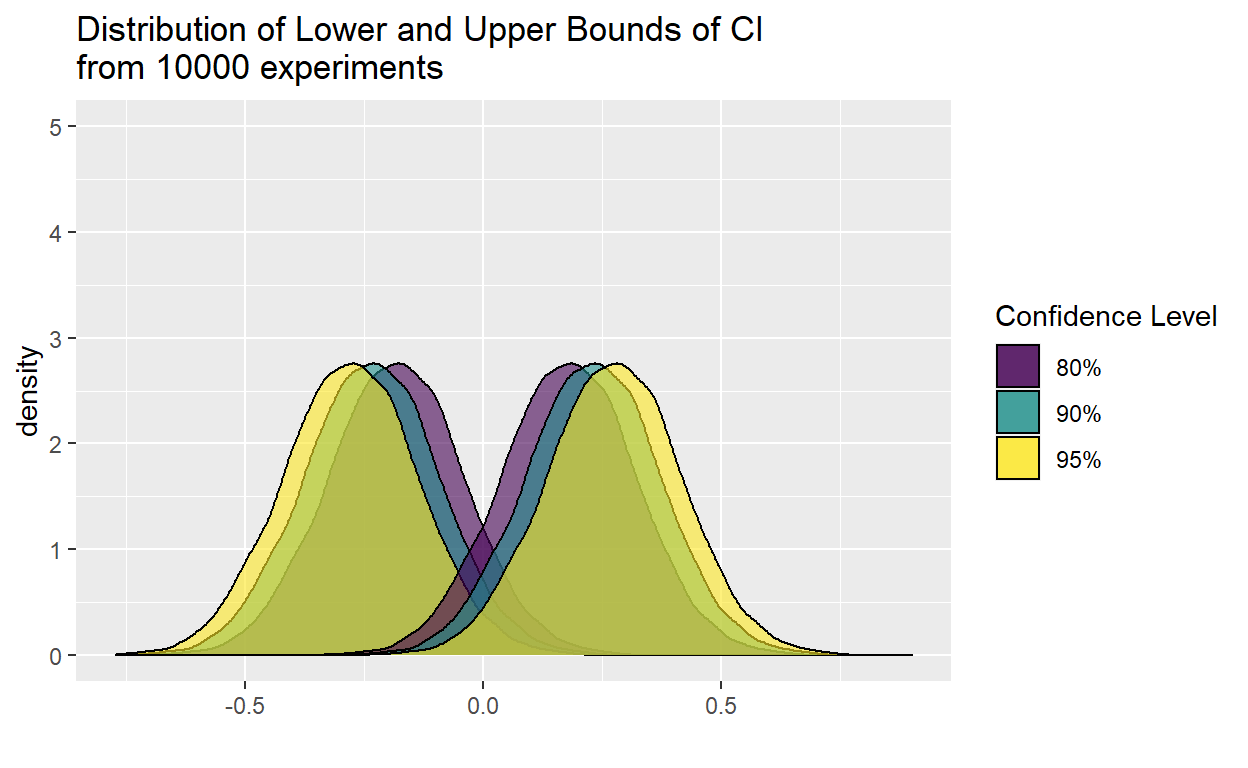
\includegraphics{a_files/figure-latex/unnamed-chunk-6-1.pdf}

\hypertarget{the-success-rate-of-intervals-with-different-confidence-levels}{%
\subsubsection{5.2 The success rate of intervals with different
confidence
levels}\label{the-success-rate-of-intervals-with-different-confidence-levels}}

The success rate of intervals also decreases as the confidence level
drops. Among 10000 experiments, we missed the true mean by 522 times
(5\% of all experiments) using 95\% confidence intervals, by 1002 times
(10\% of all experiments) using 90\% confidence intervals, and by 2015
times (20\% of all experiments) using 80\% confidence intervals.

Below is a success rate table:

\begin{Shaded}
\begin{Highlighting}[]
\FunctionTok{print}\NormalTok{(}\StringTok{"Success rate table:"}\NormalTok{)}
\end{Highlighting}
\end{Shaded}

\begin{verbatim}
## [1] "Success rate table:"
\end{verbatim}

\begin{Shaded}
\begin{Highlighting}[]
\NormalTok{rate\_table }\OtherTok{=} \FunctionTok{round}\NormalTok{(}\FunctionTok{prop.table}\NormalTok{(}\FunctionTok{table}\NormalTok{(level, if\_success), }
                              \AttributeTok{margin=}\DecValTok{1}\NormalTok{), }
                   \AttributeTok{digits =} \DecValTok{3}\NormalTok{)}
\NormalTok{rate\_table}
\end{Highlighting}
\end{Shaded}

\begin{verbatim}
##      if_success
## level Captured Missed
##   80%    0.799  0.201
##   90%    0.899  0.101
##   95%    0.948  0.052
\end{verbatim}

The results we get are consistent with the definition of confidence
level. In the long run, an n\% confidence interval will capture the true
parameters approximately n\% of the time.

\hypertarget{confidence-interval}{%
\subsubsection{5.3 95\% Confidence Interval}\label{confidence-interval}}

Below we show a density plot of the sample means from 10000 experiments.
We marked the portion that captures the true mean with a 95\% confidence
interval in green, and we paint the portion that misses the true mean in
red.

\begin{Shaded}
\begin{Highlighting}[]
\FunctionTok{create\_dis\_plot}\NormalTok{(df\_95,}
                \StringTok{"Distribution of Sample Means}\SpecialCharTok{\textbackslash{}n}\StringTok{with 10000 experiments of 50 samples}\SpecialCharTok{\textbackslash{}n}\StringTok{from a Normal Distribution (mu=0, sd=1)"}\NormalTok{,}
\NormalTok{                rate\_table[}\DecValTok{3}\NormalTok{, ])}
\end{Highlighting}
\end{Shaded}

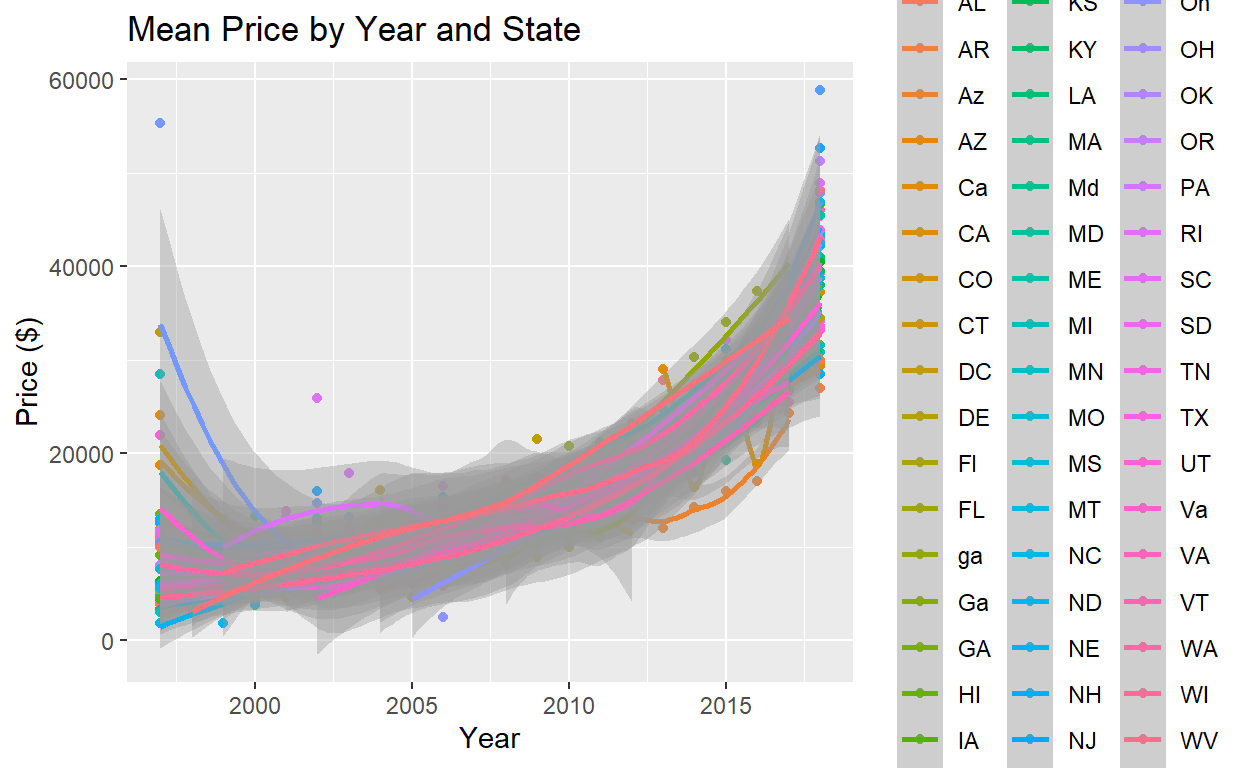
\includegraphics{a_files/figure-latex/unnamed-chunk-8-1.pdf}

As the plot shows, the distribution of sampling mean has a shape of a
normal distribution with a mean of 0. About 5.2\% of the experiments
miss the true mean using the 95\% confidence intervals.

To further investigate how confidence level affects the interval's
success rate (accuracy) and width, we create the following scatter plot
with error bars.

To generate this plot, we \textbf{randomly select 100} experiments. We
plot the sample mean of each experiment using a scatter plot and its
95\%, 90\%, and 80\% confidence intervals using error bars. The
experiments that capture the true mean (blue horizontal line) are marked
in green, and the experiments that miss the true mean are marked in red.

We fix the scale of the y axis so you can observe how the interval width
decreases as we reduce the confidence levels. You will also find more
misses when the interval width decreases.

\begin{Shaded}
\begin{Highlighting}[]
\FunctionTok{set.seed}\NormalTok{(}\DecValTok{189}\NormalTok{)}
\NormalTok{random\_100 }\OtherTok{=} \FunctionTok{sample}\NormalTok{(}\FunctionTok{nrow}\NormalTok{(df\_95), }\DecValTok{100}\NormalTok{)}
\NormalTok{df\_95\_sub }\OtherTok{=}\NormalTok{ df\_95[random\_100, ]}
\NormalTok{df\_95\_sub}\SpecialCharTok{$}\NormalTok{nth\_exp }\OtherTok{=} \DecValTok{1}\SpecialCharTok{:}\DecValTok{100}
\NormalTok{missed }\OtherTok{=} \FunctionTok{sum}\NormalTok{(df\_95\_sub}\SpecialCharTok{$}\NormalTok{if\_success }\SpecialCharTok{==} \StringTok{"Missed"}\NormalTok{)}
\NormalTok{success }\OtherTok{=} \DecValTok{100} \SpecialCharTok{{-}}\NormalTok{ missed}
\FunctionTok{create\_ci\_plot}\NormalTok{(df\_95\_sub, }
               \DecValTok{0}\NormalTok{,}
               \AttributeTok{plot\_title =} \FunctionTok{paste}\NormalTok{(}\StringTok{"95\% Confidence Interval of 100 Experiments"}\NormalTok{,}
                                  \StringTok{"}\SpecialCharTok{\textbackslash{}n}\StringTok{Missed"}\NormalTok{, missed, }\StringTok{", Success"}\NormalTok{, success),}
               \AttributeTok{ytitle =} \StringTok{"Sample Mean"}\NormalTok{,}
               \FloatTok{0.7}\NormalTok{,}
               \SpecialCharTok{{-}}\FloatTok{0.7}\NormalTok{)}
\end{Highlighting}
\end{Shaded}

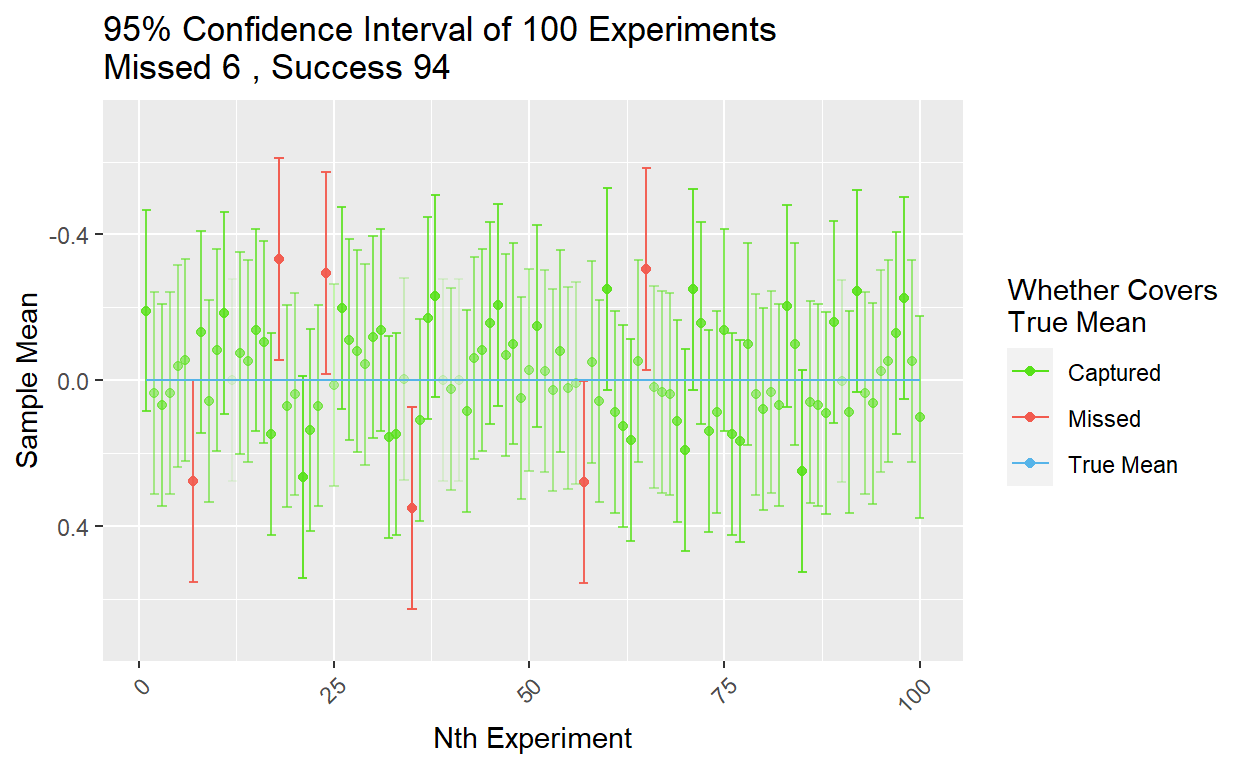
\includegraphics{a_files/figure-latex/unnamed-chunk-9-1.pdf}

We use the variable opacity (\texttt{alpha}) when plotting the
confidence interval. If the center of a confidence interval is farther
from the population mean, the confidence interval will have a higher
opacity (\texttt{alpha}). This will help us highlight the experiments in
which the confidence interval will miss the true mean if we further
decrease the confidence level.

\hypertarget{confidence-interval-1}{%
\subsubsection{5.4 90\% Confidence
Interval}\label{confidence-interval-1}}

What will happen if we drop the confidence level from 95\% to 90\%?

As shown in the sampling distribution plot below, a 90\% confidence
interval will have a lower success rate of capturing the population
mean. About 10\% of the experiments fail to capture the true mean.

\begin{Shaded}
\begin{Highlighting}[]
\NormalTok{df\_90 }\OtherTok{=}\NormalTok{ df[df}\SpecialCharTok{$}\NormalTok{confidence\_level }\SpecialCharTok{==} \StringTok{"90\%"}\NormalTok{,]}

\FunctionTok{create\_dis\_plot}\NormalTok{(df\_90, }
                \StringTok{"Distribution of Sample Means}\SpecialCharTok{\textbackslash{}n}\StringTok{with 10000 experiments of 50 samples}\SpecialCharTok{\textbackslash{}n}\StringTok{from a Normal Distribution (mu=0, sd=1)"}\NormalTok{,}
\NormalTok{                rate\_table[}\DecValTok{2}\NormalTok{, ])}
\end{Highlighting}
\end{Shaded}

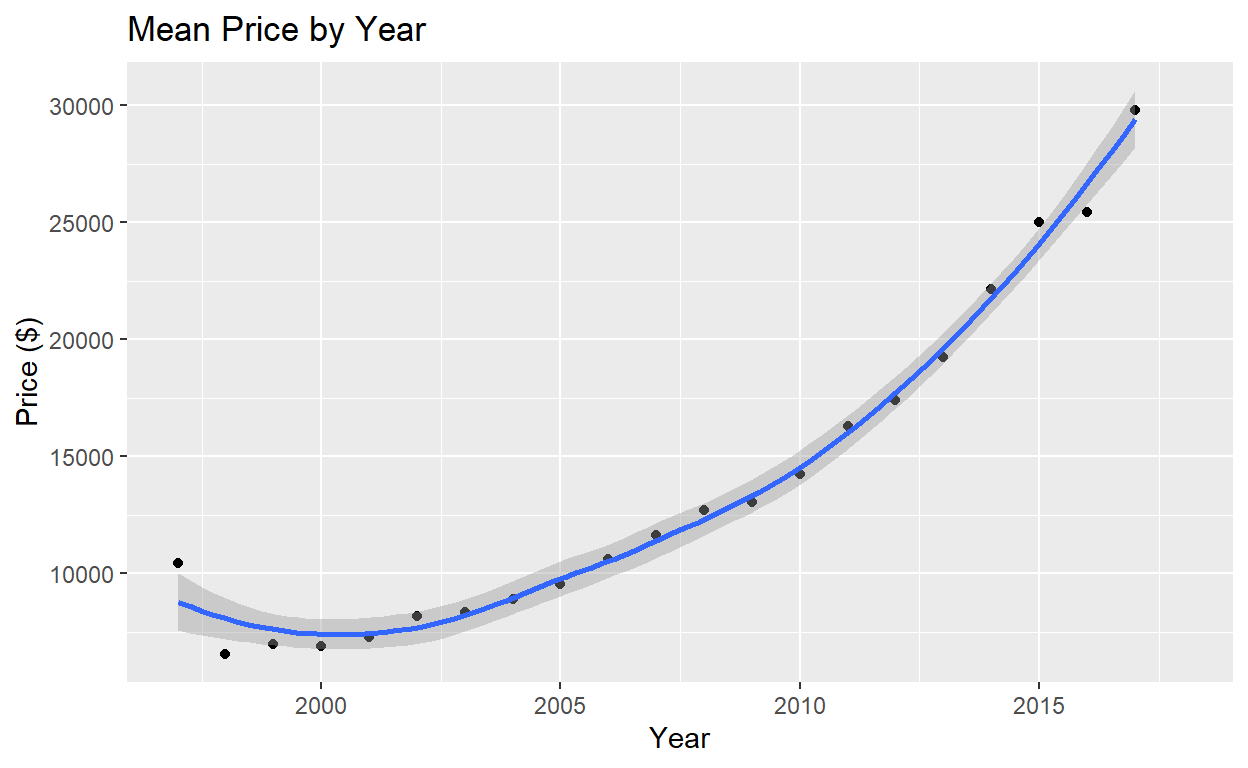
\includegraphics{a_files/figure-latex/unnamed-chunk-10-1.pdf}

The accuracy drops because the confidence interval is shrinking. Eight
more experiments that previously captured the true mean with 95\%
confidence intervals now miss it because the width of their interval
shrinks.

\begin{Shaded}
\begin{Highlighting}[]
\NormalTok{df\_90\_sub }\OtherTok{=}\NormalTok{ df\_90[random\_100, ]}
\NormalTok{df\_90\_sub}\SpecialCharTok{$}\NormalTok{nth\_exp }\OtherTok{=} \DecValTok{1}\SpecialCharTok{:}\DecValTok{100}
\NormalTok{missed }\OtherTok{=} \FunctionTok{sum}\NormalTok{(df\_90\_sub}\SpecialCharTok{$}\NormalTok{if\_success }\SpecialCharTok{==} \StringTok{"Missed"}\NormalTok{)}
\NormalTok{success }\OtherTok{=} \DecValTok{100} \SpecialCharTok{{-}}\NormalTok{ missed}
\FunctionTok{create\_ci\_plot}\NormalTok{(df\_90\_sub, }
               \DecValTok{0}\NormalTok{,}
               \AttributeTok{plot\_title =} \FunctionTok{paste}\NormalTok{(}\StringTok{"90\% Confidence Interval of 100 Experiments"}\NormalTok{,}
                                  \StringTok{"}\SpecialCharTok{\textbackslash{}n}\StringTok{Missed"}\NormalTok{, missed, }\StringTok{", Success"}\NormalTok{, success),}
               \AttributeTok{ytitle =} \StringTok{"Sample Mean"}\NormalTok{,}
               \FloatTok{0.7}\NormalTok{,}
               \SpecialCharTok{{-}}\FloatTok{0.7}\NormalTok{)}
\end{Highlighting}
\end{Shaded}

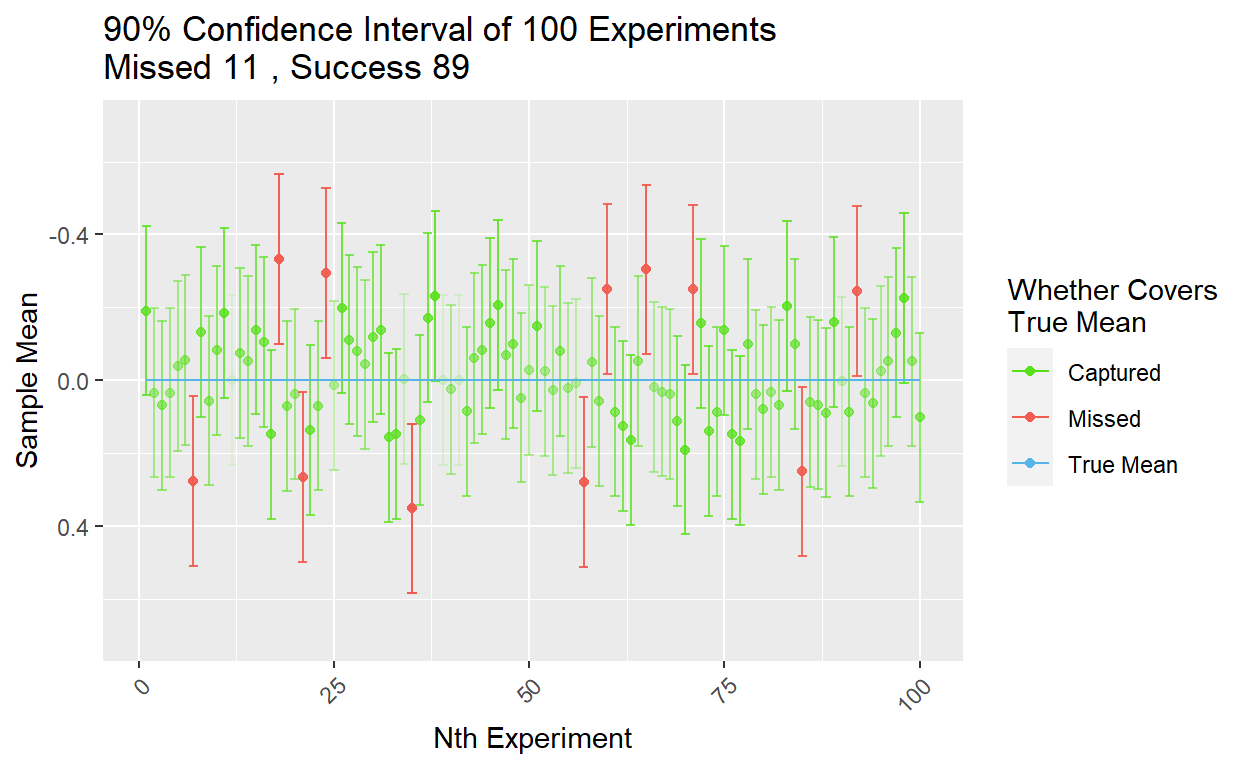
\includegraphics{a_files/figure-latex/unnamed-chunk-11-1.pdf}

\hypertarget{confidence-interval-2}{%
\subsubsection{5.5 80\% Confidence
Interval}\label{confidence-interval-2}}

As we keep decreasing the confidence level, about 2000 out of 10000
experiments now miss the true mean with their 80\% confidence interval.

\begin{Shaded}
\begin{Highlighting}[]
\NormalTok{df\_80 }\OtherTok{=}\NormalTok{ df[df}\SpecialCharTok{$}\NormalTok{confidence\_level }\SpecialCharTok{==} \StringTok{"80\%"}\NormalTok{,]}

\FunctionTok{create\_dis\_plot}\NormalTok{(df\_80, }
                \StringTok{"Distribution of Sample Means}\SpecialCharTok{\textbackslash{}n}\StringTok{with 10000 experiments of 50 samples}\SpecialCharTok{\textbackslash{}n}\StringTok{from a Normal Distribution (mu=0, sd=1)"}\NormalTok{, }
\NormalTok{                rate\_table[}\DecValTok{1}\NormalTok{, ])}
\end{Highlighting}
\end{Shaded}

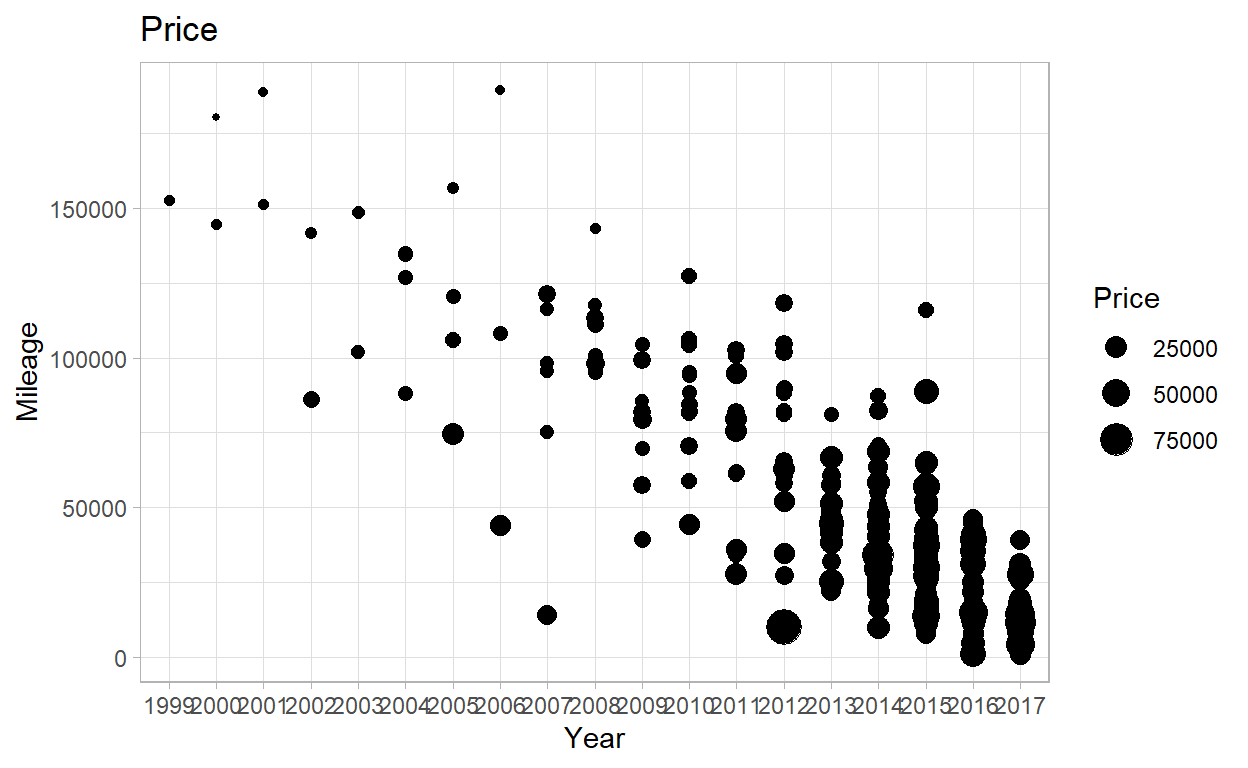
\includegraphics{a_files/figure-latex/unnamed-chunk-12-1.pdf}

The width of the confidence interval also decreases. For the same 100
randomly selected experiments, 19 of them miss the true mean as their
interval width shrinks.

\begin{Shaded}
\begin{Highlighting}[]
\NormalTok{df\_80\_sub }\OtherTok{=}\NormalTok{ df\_80[random\_100, ]}
\NormalTok{df\_80\_sub}\SpecialCharTok{$}\NormalTok{nth\_exp }\OtherTok{=} \DecValTok{1}\SpecialCharTok{:}\DecValTok{100}
\NormalTok{missed }\OtherTok{=} \FunctionTok{sum}\NormalTok{(df\_80\_sub}\SpecialCharTok{$}\NormalTok{if\_success }\SpecialCharTok{==} \StringTok{"Missed"}\NormalTok{)}
\NormalTok{success }\OtherTok{=} \DecValTok{100} \SpecialCharTok{{-}}\NormalTok{ missed}
\FunctionTok{create\_ci\_plot}\NormalTok{(df\_80\_sub, }
               \DecValTok{0}\NormalTok{,}
               \AttributeTok{plot\_title =} \FunctionTok{paste}\NormalTok{(}\StringTok{"80\% Confidence Interval of 100 Experiments"}\NormalTok{,}
                                  \StringTok{"}\SpecialCharTok{\textbackslash{}n}\StringTok{Missed"}\NormalTok{, missed, }\StringTok{", Success"}\NormalTok{, success),}
               \AttributeTok{ytitle =} \StringTok{"Sample Mean"}\NormalTok{,}
               \FloatTok{0.7}\NormalTok{,}
               \SpecialCharTok{{-}}\FloatTok{0.7}\NormalTok{)}
\end{Highlighting}
\end{Shaded}

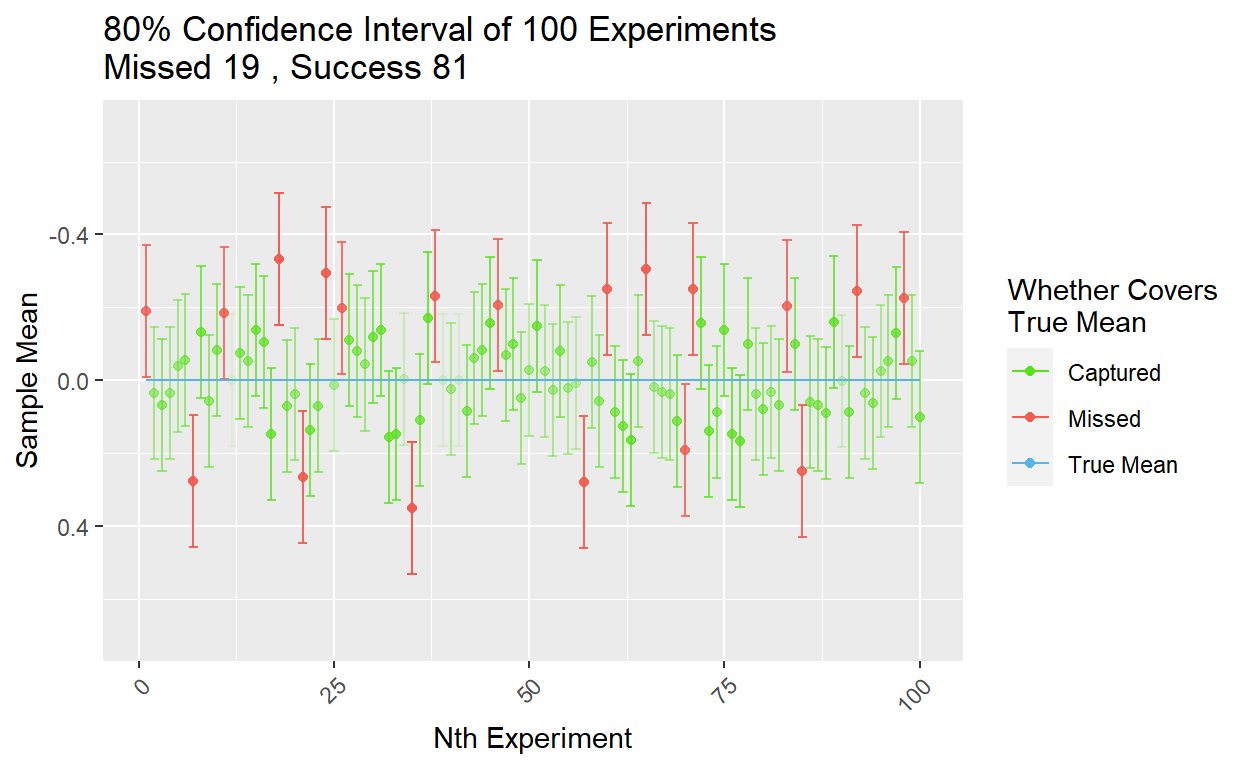
\includegraphics{a_files/figure-latex/unnamed-chunk-13-1.pdf}

\hypertarget{confidence-levels-effect-on-interval-width}{%
\subsubsection{5.6 Confidence Level's Effect on Interval
Width}\label{confidence-levels-effect-on-interval-width}}

Let's look closely at the confidence level's effect on interval width.
We randomly select 6 experiments and plot their 95\%, 90\%, and 80\%
confidence intervals in pastel purple, pastel yellow, and mint brackets
respectively. We scale the widths of brackets based on their confidence
levels so you can directly observe their difference even if they are
overlaid.

\begin{Shaded}
\begin{Highlighting}[]
\NormalTok{random\_exp }\OtherTok{=} \FunctionTok{sample}\NormalTok{(}\DecValTok{1}\SpecialCharTok{:}\NormalTok{num\_exp, }\DecValTok{6}\NormalTok{)}
\NormalTok{random\_exp }\OtherTok{=} \FunctionTok{c}\NormalTok{(random\_exp, }
\NormalTok{               random\_exp }\SpecialCharTok{+}\NormalTok{ num\_exp,}
\NormalTok{               random\_exp }\SpecialCharTok{+} \DecValTok{2} \SpecialCharTok{*}\NormalTok{ num\_exp)}
\NormalTok{df\_sub }\OtherTok{=}\NormalTok{ df[random\_exp,]}
\NormalTok{df\_sub }\OtherTok{=}\NormalTok{ df\_sub[}\FunctionTok{nrow}\NormalTok{(df\_sub)}\SpecialCharTok{:}\DecValTok{1}\NormalTok{,]}
\NormalTok{df\_sub}\SpecialCharTok{$}\NormalTok{nth\_exp }\OtherTok{=} \FunctionTok{rep}\NormalTok{(}\DecValTok{1}\SpecialCharTok{:}\DecValTok{6}\NormalTok{, }\AttributeTok{times=}\DecValTok{3}\NormalTok{)}

\NormalTok{p }\OtherTok{\textless{}{-}} \FunctionTok{ggplot}\NormalTok{(}\AttributeTok{data=}\NormalTok{df\_sub, }\FunctionTok{aes}\NormalTok{(}\AttributeTok{y=}\NormalTok{nth\_exp, }\AttributeTok{x=}\NormalTok{sample\_mean)) }\SpecialCharTok{+}
      \FunctionTok{geom\_point}\NormalTok{(}\AttributeTok{size=}\DecValTok{4}\NormalTok{) }\SpecialCharTok{+}
      \FunctionTok{geom\_errorbar}\NormalTok{(}\FunctionTok{aes}\NormalTok{(}\AttributeTok{xmin=}\NormalTok{lb, }\AttributeTok{xmax=}\NormalTok{ub, }
                        \AttributeTok{color=}\NormalTok{confidence\_level,}
                        \AttributeTok{size=}\NormalTok{confidence\_level), }
                    \AttributeTok{width=}\FloatTok{0.5}\NormalTok{, }\AttributeTok{alpha=}\FloatTok{0.9}\NormalTok{) }\SpecialCharTok{+}
      \FunctionTok{geom\_line}\NormalTok{(}\FunctionTok{aes}\NormalTok{(}\AttributeTok{y=}\NormalTok{nth\_exp, }\AttributeTok{x=}\NormalTok{pop\_mean, }
                    \AttributeTok{color=}\StringTok{"True Mean"}\NormalTok{),}
                \AttributeTok{size=}\DecValTok{2}\NormalTok{) }\SpecialCharTok{+}
      \FunctionTok{xlab}\NormalTok{(}\StringTok{"Sample Mean"}\NormalTok{) }\SpecialCharTok{+}
      \FunctionTok{ylab}\NormalTok{(}\StringTok{"Nth Experiment"}\NormalTok{) }\SpecialCharTok{+}
      \FunctionTok{labs}\NormalTok{(}\AttributeTok{title=}\StringTok{"Confidence Level\textquotesingle{}s Effect on}\SpecialCharTok{\textbackslash{}n}\StringTok{Interval Width"}\NormalTok{,}
           \AttributeTok{color =} \StringTok{"Confidence Level"}\NormalTok{) }\SpecialCharTok{+}
      \FunctionTok{guides}\NormalTok{(}\AttributeTok{size=}\StringTok{"none"}\NormalTok{) }\SpecialCharTok{+}
      \FunctionTok{scale\_size\_manual}\NormalTok{(}\AttributeTok{values=}\FunctionTok{c}\NormalTok{(}\DecValTok{1}\NormalTok{, }\DecValTok{2}\NormalTok{, }\DecValTok{3}\NormalTok{)) }\SpecialCharTok{+}
      \FunctionTok{scale\_color\_brewer}\NormalTok{(}\AttributeTok{palette =} \StringTok{"Set3"}\NormalTok{)}
\NormalTok{p }\SpecialCharTok{+} \FunctionTok{aes}\NormalTok{(}\AttributeTok{group=}\FunctionTok{rev}\NormalTok{(confidence\_level))}
\end{Highlighting}
\end{Shaded}

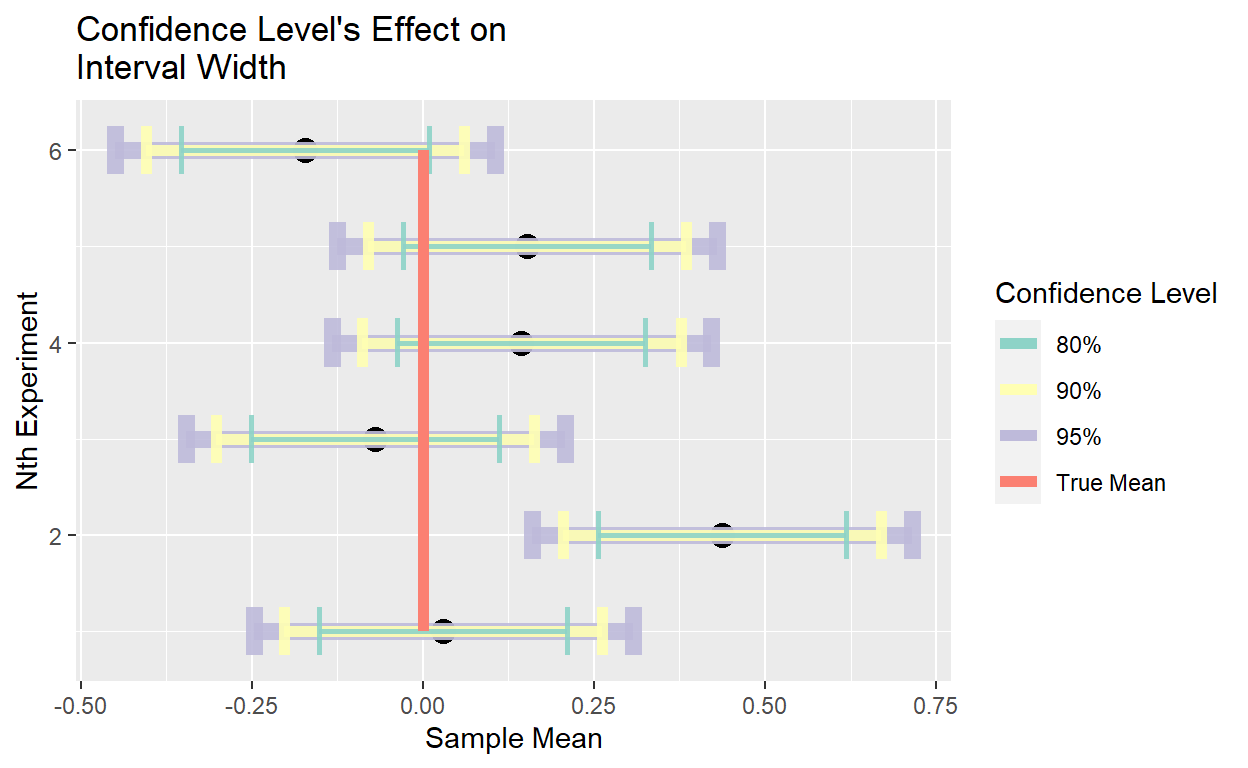
\includegraphics{a_files/figure-latex/unnamed-chunk-14-1.pdf}

\begin{Shaded}
\begin{Highlighting}[]
\FunctionTok{ggsave}\NormalTok{(}\StringTok{"df\_sub.png"}\NormalTok{)}
\end{Highlighting}
\end{Shaded}

\begin{verbatim}
## Saving 6.5 x 4.5 in image
\end{verbatim}

We can observe that the width of the interval increases as the
confidence level becomes higher. This is expected because a wider width
interval will have a higher frequency of covering the true parameter in
the long run. As we learned from the previous scatter plots of 100
experiments, more experiments missed the true mean when their confidence
intervals became narrower.

\hypertarget{future-work}{%
\subsection{6. Future Work}\label{future-work}}

We will turn the visualizations of the sampling distributions and
confidence intervals plots (sec 5.3) into interactive applications in
the next stage of this project.

Below are a few sketches of our application designs:

\begin{figure}
\centering
\includegraphics{image1.jpg}
\caption{Application Design}
\end{figure}

Confidence Interval Plots: Our design of the interactive confidence
interval plots is in the upper part of our sketch. For this
visualization, we will have a slide bar to allow users to adjust the
confidence level and see how it affects the interval width (shrinking or
enlarging) and the success rate (more or fewer intervals cover the true
mean).

Sampling Distribution Plots: Our design of the sampling distribution
plots is in the lower part of our sketch. For this visualization, we
will have two slide bars (or input boxes) for users to adjust the sample
size, \(n\), and population standard deviation, \(\sigma\). This will
help users to visualize how \(n\) and \(\sigma\) affect the shape of a
sampling distribution as illustrated in the central limit theorem. We
will also have a slide bar for the confidence level. The proportion of
the sample means of which the associated intervals to capture the true
parameter will be shaded in red. As users adjust the confidence level,
they will observe how the red area shrinks or enlarges proportionally
with the new confidence level.

\hypertarget{real-life-usage-examples}{%
\subsection{7. Real Life Usage \&
Examples}\label{real-life-usage-examples}}

Remember that confidence intervals are used to give a range as an
estimate for an unknown population parameter, which is often the mean or
the standard deviation. In real life, confidence intervals are used a
lot when we try to gain insight into properties, like the mean and the
SD, about the population in a cost-efficient way or when taking a census
(sampling every individual in the population) isn't possible.

Example 1: Biology Confidence intervals are often used in biology to
estimate the mean height, weight, width, diameter, etc. of different
plant and animal species. For example, a biologist may be interested in
measuring the mean weight of a certain species of frog in Australia.
Since it would take too long to go around and weigh thousands of
individual frogs, the biologist may instead collect a simple random
sample of 50 frogs and measure the mean and standard deviation of the
frogs in the sample. She could then use the sample mean and sample
standard deviation to construct an interval for the true mean of the
frogs in the entire population.

Example 2: Clinical Trials Confidence intervals are often used in
clinical trials to determine the mean change in blood pressure, heart
rate, cholesterol, etc. produced by some new drug or treatment. For
example, a doctor may believe that a new drug is able to reduce blood
pressure in patients. To test this, he may recruit 20 patients to
participate in a trial in which they used the new drug for one month. At
the end of the month, the doctor may record the mean decrease in blood
pressure and the standard deviation of the decrease in each patient in
the sample. 15 Students Weekday Sleep (hours) 0 25 50 75 100 He could
then use the sample mean and sample standard deviation to construct an
interval for the true mean change in blood pressure that patients are
likely to experience in the population.

Example 3: Polling Confidence intervals are used in polling to gauge
voter support for laws or taxes at the local, state, or national level.
Let's say we want to find the percentage of city voters that support a
property tax increase to build a new police station. To save time, we
can poll a small group of citizens (rather than the entire city's
population) and find a confidence interval. Using a 95\% confidence
interval, we might find a range of (62\%, 68\%). This can tell us that,
with 95\% confidence, a majority (more than 50\%) of the city's voters
support certain policies.

References:\\
\url{https://www.statology.org/confidence-interval-real-life-example/}\strut \\
\href{https://www.statology.org/confidence-interval-real-life-example/}{https://www.quora.com/Where-
are-confidence-intervals-used-in-real-life}

\begin{Shaded}
\begin{Highlighting}[]
\FunctionTok{library}\NormalTok{(ggplot2)}

\CommentTok{\# Inter{-}arival Time Dist {-} Exp(rate=.50286)}
\FunctionTok{ggplot}\NormalTok{() }\SpecialCharTok{+}
  \FunctionTok{xlim}\NormalTok{(}\DecValTok{0}\NormalTok{, }\DecValTok{8}\NormalTok{) }\SpecialCharTok{+}
  \FunctionTok{stat\_function}\NormalTok{(}\AttributeTok{fun =}\NormalTok{ dexp,}
                \AttributeTok{args =} \FunctionTok{list}\NormalTok{(}\AttributeTok{rate =}\NormalTok{ .}\DecValTok{50286}\NormalTok{),}
                \AttributeTok{geom =} \StringTok{"area"}\NormalTok{,}
                \AttributeTok{fill=}\StringTok{"\#345beb"}\NormalTok{, }\AttributeTok{alpha=}\FloatTok{0.7}\NormalTok{) }\SpecialCharTok{+}
  \FunctionTok{ggtitle}\NormalTok{(}\StringTok{"Theoritical Probability Distribution Function of }\SpecialCharTok{\textbackslash{}n}\StringTok{ Exponential With Rate=0.50286"}\NormalTok{) }\SpecialCharTok{+}
  \FunctionTok{ylab}\NormalTok{(}\StringTok{"Probability"}\NormalTok{) }\SpecialCharTok{+}
  \FunctionTok{xlab}\NormalTok{(}\StringTok{"x"}\NormalTok{)}
\end{Highlighting}
\end{Shaded}

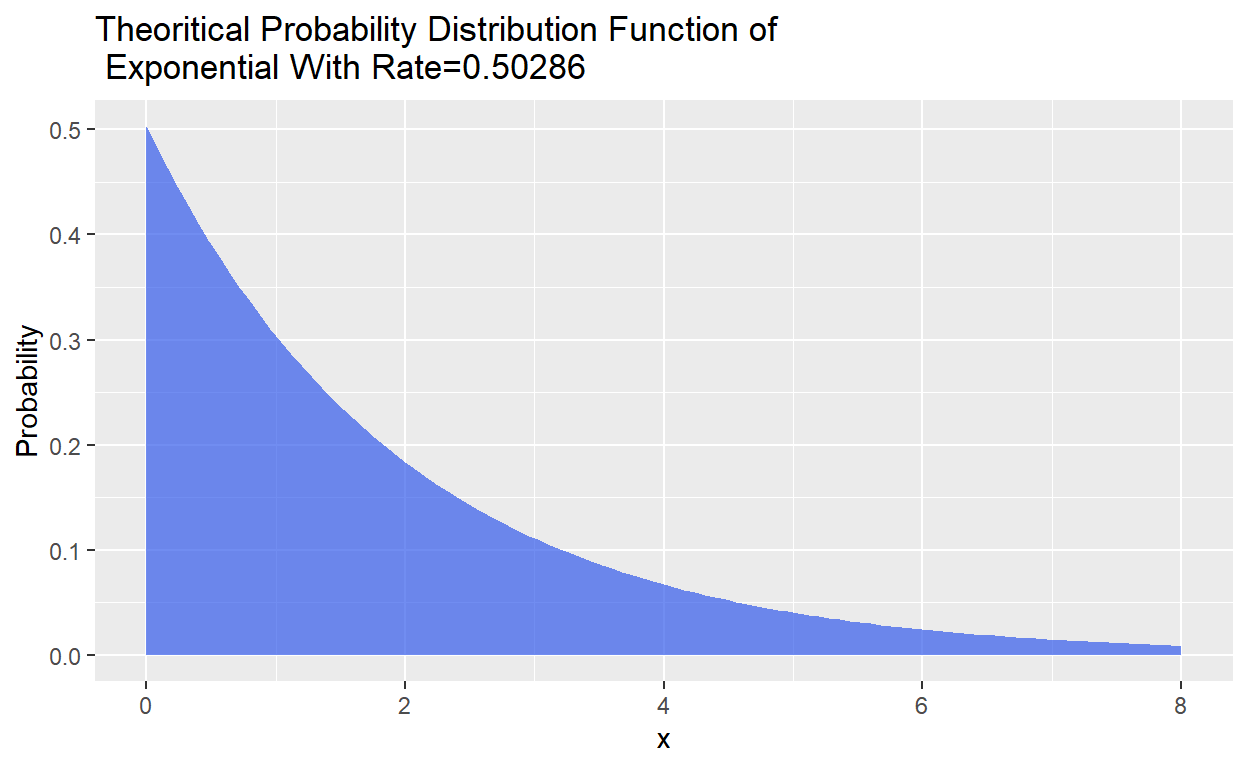
\includegraphics{a_files/figure-latex/unnamed-chunk-15-1.pdf}

\begin{Shaded}
\begin{Highlighting}[]
\FunctionTok{ggsave}\NormalTok{(}\StringTok{"expo\_dist.png"}\NormalTok{)}
\end{Highlighting}
\end{Shaded}

\begin{verbatim}
## Saving 6.5 x 4.5 in image
\end{verbatim}

\begin{Shaded}
\begin{Highlighting}[]
\NormalTok{dgamma2 }\OtherTok{\textless{}{-}} \ControlFlowTok{function}\NormalTok{(x, shape, scale) \{}
  \FunctionTok{return}\NormalTok{(}\FunctionTok{dgamma}\NormalTok{(x}\FloatTok{{-}0.1}\NormalTok{, }\AttributeTok{shape=}\NormalTok{shape, }\AttributeTok{scale=}\NormalTok{scale))}
\NormalTok{\}}

\CommentTok{\# Service Time Dist}

\FunctionTok{ggplot}\NormalTok{() }\SpecialCharTok{+}
  \FunctionTok{stat\_function}\NormalTok{(}\AttributeTok{fun =}\NormalTok{ dgamma2,}
                \AttributeTok{args =} \FunctionTok{list}\NormalTok{(}\AttributeTok{shape =} \FloatTok{2.3}\NormalTok{, }\AttributeTok{scale=}\NormalTok{.}\DecValTok{1}\NormalTok{),}
                \AttributeTok{geom =} \StringTok{"area"}\NormalTok{,}
                \AttributeTok{fill=}\StringTok{"\#345beb"}\NormalTok{, }\AttributeTok{alpha=}\FloatTok{0.7}\NormalTok{) }\SpecialCharTok{+}
  \FunctionTok{ggtitle}\NormalTok{(}\StringTok{"Therotical Probability Distribution Function of Gamma with}\SpecialCharTok{\textbackslash{}n}\StringTok{ Offset=0.1, Shape=2.3, Scale=0.1"}\NormalTok{) }\SpecialCharTok{+}
  \FunctionTok{xlab}\NormalTok{(}\StringTok{"x"}\NormalTok{) }\SpecialCharTok{+}
  \FunctionTok{ylab}\NormalTok{(}\StringTok{"Probability"}\NormalTok{)}
\end{Highlighting}
\end{Shaded}

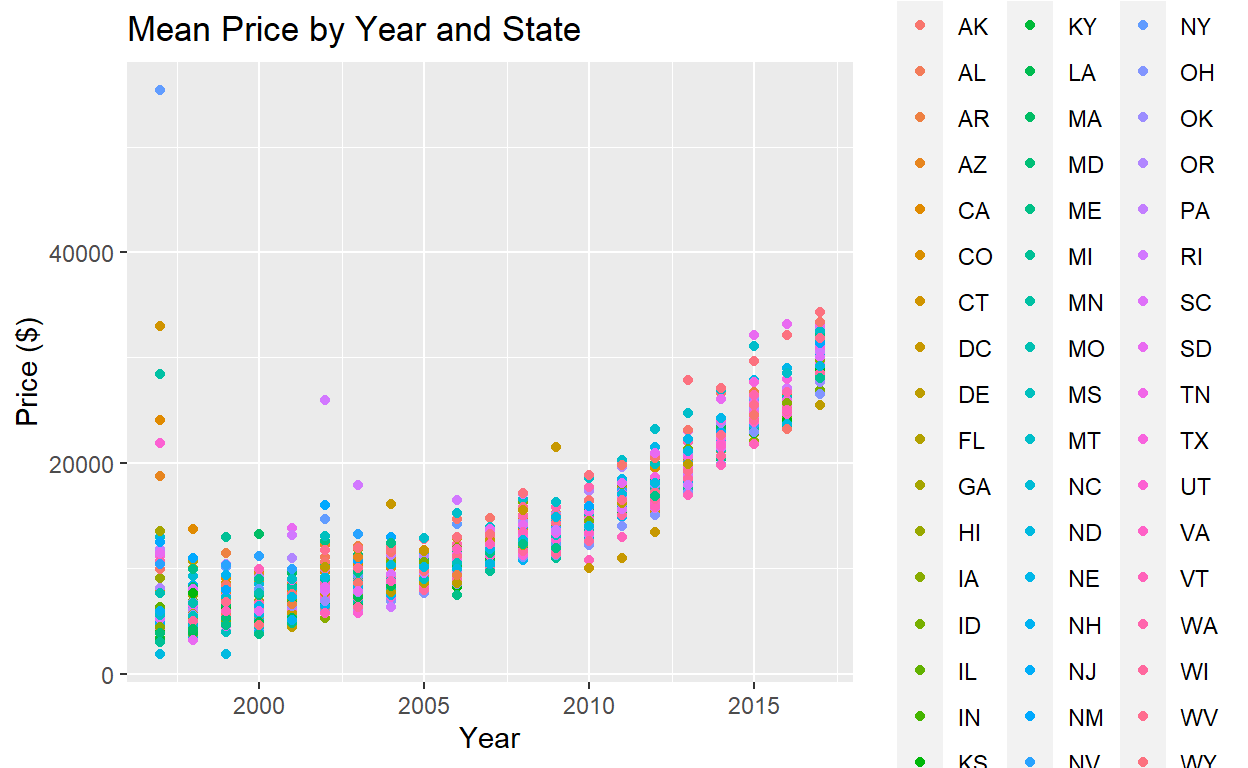
\includegraphics{a_files/figure-latex/unnamed-chunk-15-2.pdf}

\begin{Shaded}
\begin{Highlighting}[]
\FunctionTok{ggsave}\NormalTok{(}\StringTok{"gamma\_dist.png"}\NormalTok{)}
\end{Highlighting}
\end{Shaded}

\begin{verbatim}
## Saving 6.5 x 4.5 in image
\end{verbatim}

\begin{Shaded}
\begin{Highlighting}[]
\FunctionTok{curve}\NormalTok{(}\FunctionTok{dgamma2}\NormalTok{(x}\FloatTok{{-}0.1}\NormalTok{, }\AttributeTok{shape =} \FloatTok{2.3}\NormalTok{, }\AttributeTok{scale=}\NormalTok{.}\DecValTok{1}\NormalTok{), }\AttributeTok{from=}\DecValTok{0}\NormalTok{, }\AttributeTok{to=}\DecValTok{1}\NormalTok{, }\AttributeTok{col=}\StringTok{\textquotesingle{}blue\textquotesingle{}}\NormalTok{) }
\end{Highlighting}
\end{Shaded}

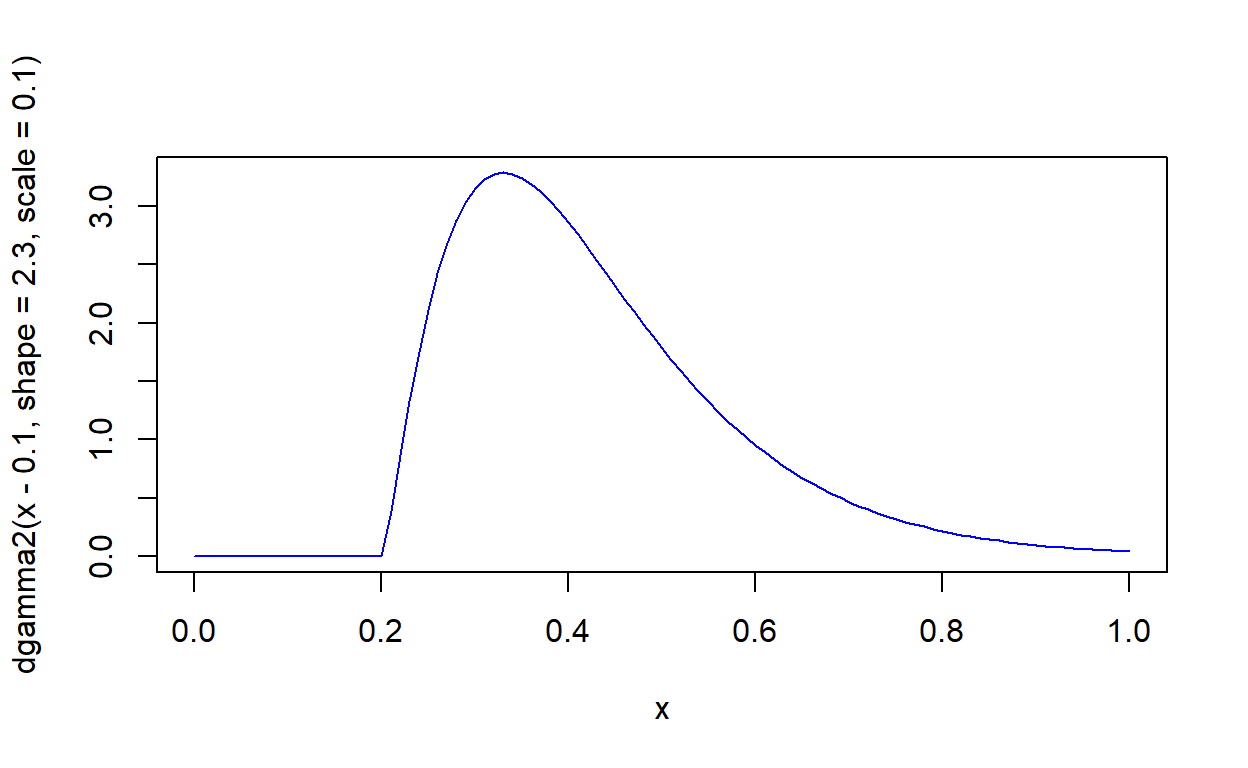
\includegraphics{a_files/figure-latex/unnamed-chunk-15-3.pdf}

\end{document}
